\chapter{Visual Design}

Visualizing syntenic data is a multi faceted problem as not only can the visual representation change based on the underlying biological question but also the resolution at which the data is being visualized.In designing a solution for this problem the taxonomy of design space created by previous synteny visualizers like Mizbee \cite{Meyer2009} was adopted and further enhanced with our recommendations for representing synteny in multi way comparisons.Two basic forms of visual representations were developed and adapted to work across multiple data resolution levels.We also adopted the visual information seeking mantra of overview,zoom and filter for exploration of data across different scales by presenting the visualizations in multiple tiers. To reduce cognitive load further we built a coordinated multiple view offering alternative representations of the same underlying data simultaneously.

\section{Visual Encoding}

A common way to represent sequence alignment or similarity is to visualize it as a two dimensional `dot plot' \cite{SONNHAMMER1995GC1,Cabanettes2018} through positional encoding.We adopted this strategy for our first visual representation by placing the source and target genomes along the \textit{x} and \textit{y} axes respectively and marking gene alignments with dots as shown in Figure \ref{fig:ch_4_dot_plot_a}.Grid-lines were then further added to the plot to indicate chromosomal boundaries.

\begin{figure}[h]
  \centering
  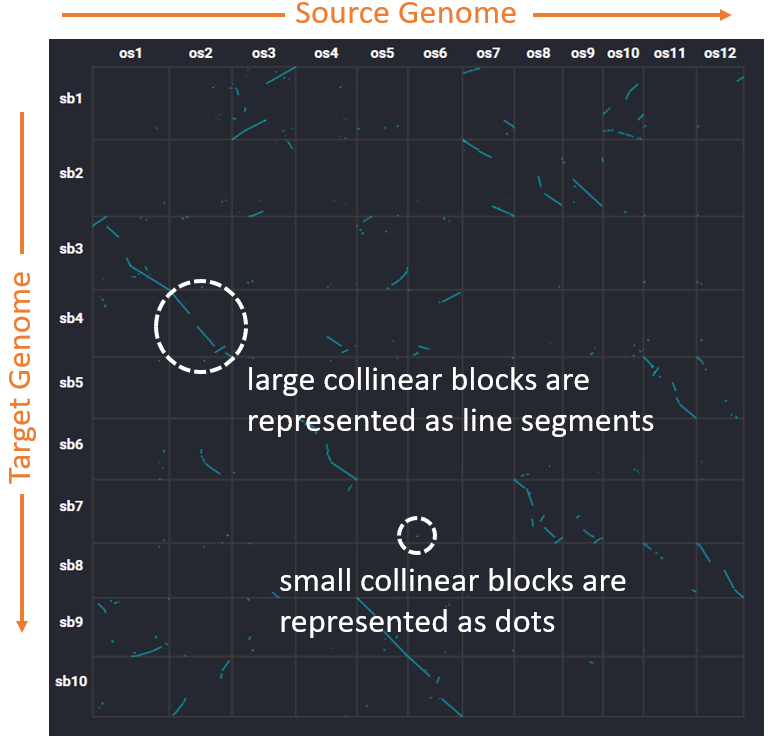
\includegraphics[width=.475\linewidth]{images/ch_4_dot_plot_a.PNG}
  \captionof{figure}{Dot plot showing whole genome synteny between Oriza sativa(rice) and Sorghum bicolor(corn) with grid-lines added for chromosomal boundaries.}
  \label{fig:ch_4_dot_plot_a}
\end{figure}

This plot can also be adopted for other resolutions by changing the genomes along \textit{x,y} axes to either individual chromosomes or smaller gene blocks.Such matrix based representations are very good at providing an overview of the dataset and can be used to highlight breaks, inversions and duplications as shown in Figure \ref{fig:ch_4_dot_plot_b}.However being a fairly primitive visual representation dot plots are often found to be visually unappealing and complex to understand without the proper background context making them unsuitable for scientific publications compared to other alternatives.


\begin{figure}
  \centering
  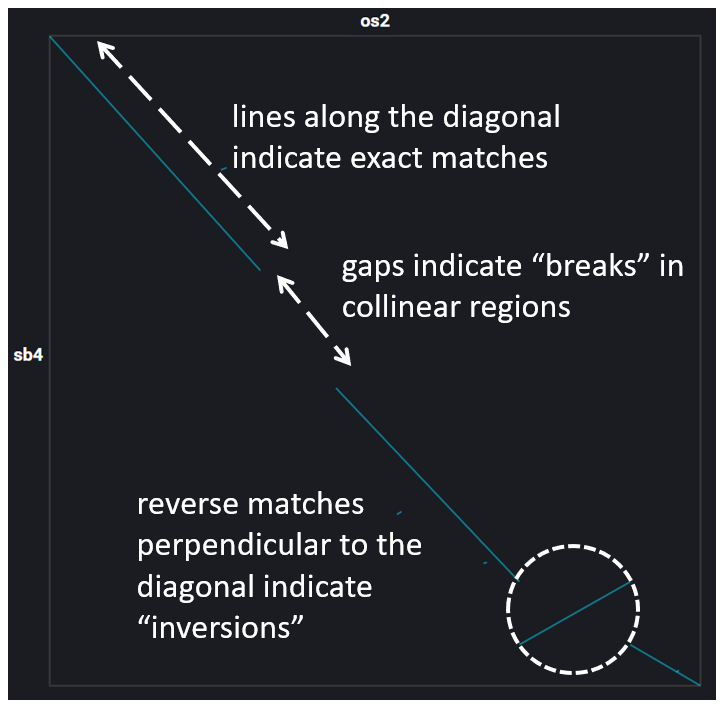
\includegraphics[width=.475\linewidth]{images/ch_4_dot_plot_b.PNG}
  \captionof{figure}{Dot plot showing breaks,inversions and duplication events between chromosome 2 and 4 of Oriza Sativa(rice) and Sorghum Bicolor(corn) respectively.}
  \label{fig:ch_4_dot_plot_b}
\end{figure}


For our second basic visual representation we adopt a design that represents synteny through a combination of positional encoding for genomic distances and connected lines for similarity.In this approach genomic sequences are stacked horizontally and similar genes are connected through lines to indicate similarity.However, unlike dot plots which use the same visual encoding across all genomic sizes for this visual representation we adopt a different secondary encoding based on the resolution of the genomic sequences being visualized. 


There are three basic levels in which synteny can be visualized starting from the gene block level which is the smallest unit at which syntenic data is reported.It is a collection of collinear genes in the source genome that are aligned to a group of collinear genes in the target genome.To encode conservation at this level, two gene blocks are represented by line segments that are stacked parallel to each other and similar genes within the blocks are connected with ribbons as shown in figure.The length of the connecting ribbon is based on the number of base pairs in the matching genes.The source and target gene blocks are annotated with numeric tracks corresponding to their position in the chromosome and are coloured in distinct colors to distinguish them.The individual genes are highlighted with a deeper shade of the base colour of the track for easier reference. 

\begin{figure}
  \centering
  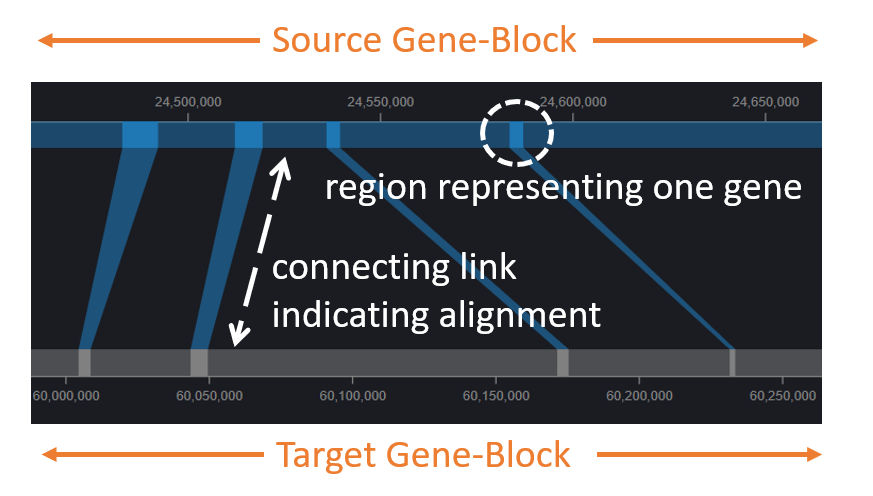
\includegraphics[width=.50\linewidth]{images/ch_4_link_plot.PNG}
  \captionof{figure}{Link Plot at the Gene-block Level}
  \label{fig:ch_4_link_plot}
\end{figure}



At the next level individual chromosomes are considered since gene blocks are internally smaller segments within a chromosome.Visualizing synteny at this level involves encoding information related to the location,size and orientation of conserved regions.To achieve this chromosomes are stacked parallel to each other and their lengths are encoded to reflect their genomic size and so chromosomes with more base-pairs in them show up as longer line segments.conserved regions in the chromosomes are then connected through ribbons from their positions on the chromosome to indicate similarity.This encodes both the location and the size of the of the conserved regions as the width of ribbons changes based on the genomic size of the linked gene blocks.


\begin{figure}[h]
  \centering
  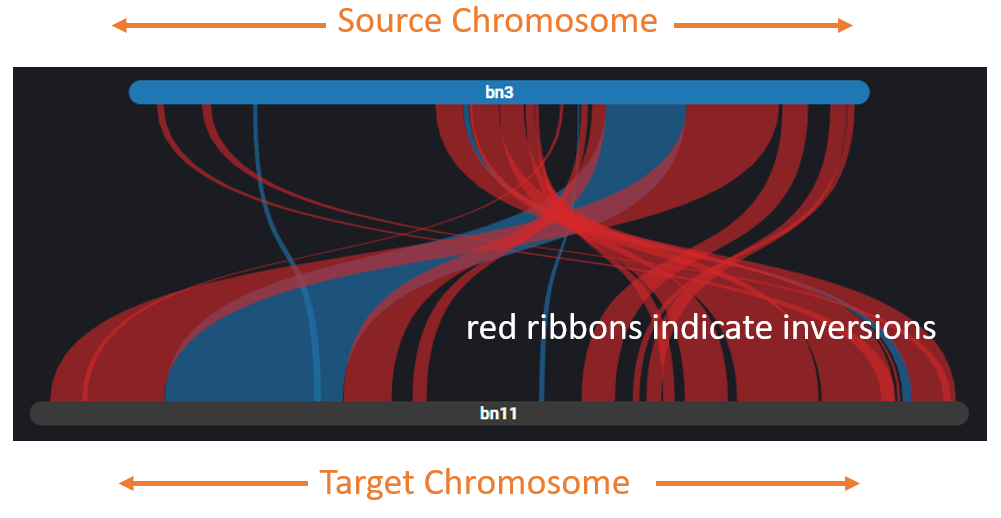
\includegraphics[width=.50\linewidth]{images/ch_4_link_plot_chromosome_a.PNG}
  \captionof{figure}{Link Plot at the Chromosome level where the blue coloured ribbons represent forward matches and the red coloured ribbons represent reverse matches(inversions).}
  \label{fig:ch_4_link_plot_chromosome_a}
\end{figure}


To encode orientation of the gene block secondary encoding in the form of colour is adopted to visual distinguish gene inversions as shown in figure \ref{fig:ch_4_link_plot_chromosome_a}.So forward matches are coloured in blue and reverse matches are coloured in red.Unlike the gene block level, at the chromosome level several bands can overlap and cross each other due to multiple gene translocation and inversions events and can cause visual clutter.To mitigate this problem complex polygons are used instead of rectangular ribbons and are generated through \textbf{B}-spline curves\cite{ref851370272} with control points set to bundle the curves towards the centre.The control points points are set vertically in the middle of the parallel blocks to ensure that the original size of the ribbons remain undistorted at regions where they join the chromosome as they visually represent the size of the conserved region as shown in figure \ref{fig:ch_4_link_plot_chromosome_b}. 

\begin{figure}
  \centering
  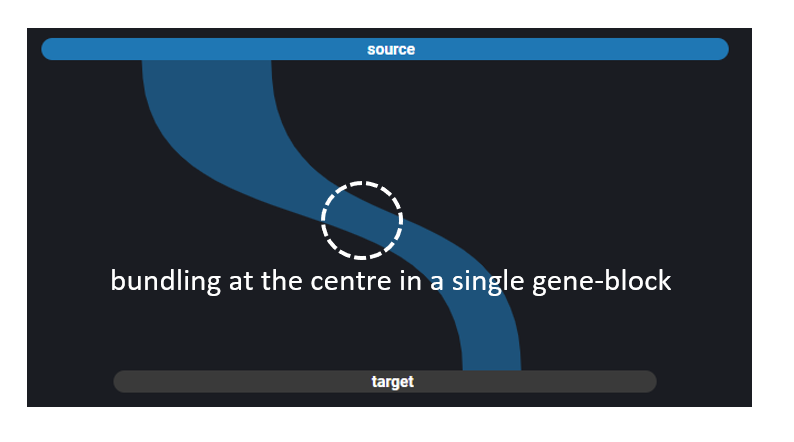
\includegraphics[width=.50\linewidth]{images/ch_4_link_plot_chromosome_b.PNG}
  \captionof{figure}{Ribbon bundling to reduce visual clutter with the control points set towards the centre indicated in a single gene-block.}
  \label{fig:ch_4_link_plot_chromosome_b}
\end{figure}


Finally at the whole genome level where syteny is observed between several chromosomes at once, smaller details such as inversions have less precedence and so the secondary encoding in the form of colour is used to distinguish different chromosomes instead of the orientation of the syntenic region.A layout similar to the parallel stacking at chromosome level is adopted however instead of having a single connected unit for the entire genome chromosomes are separated from each other with gaps serving to indicate the start and end of each chromosome.Chromosomes in the source layer are assigned a unique color while chromosomes in the target layer are assigned an alternate gray coloring scheme.Ribbons are then linked between conserved regions to represent syntenic gene-blocks and are assigned a color based on their source chromosome.This form of encoding location information about the source in the connection through colour has been used earlier in other syteny visualisations systems and has been proved effective \cite{Meyer2009}.We adopt the aforementioned bundling strategy of using \textbf{B}-spline curves\cite{ref851370272} to improve visual clarity but set the control points independently for every chromosome to group all the gene blocks emerging from each chromosome into a single bundle.


\begin{figure}
  \centering
  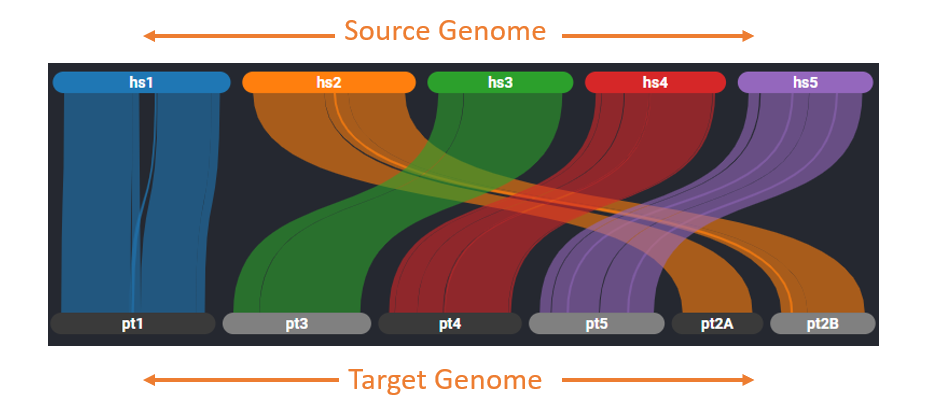
\includegraphics[width=.75\linewidth]{images/ch_4_genome_level.PNG}
  \captionof{figure}{Visual encoding at the chromosome level with connecting ribbons coloured based on the source chromosome they are linked from.}
  \label{fig:ch_4_genome_level}
\end{figure}



\section{Layout Strategies}

A common strategy that is used among all the three parallel stacked representations is the vertical separation between the source and the target to visually distinguish the two regions.This is easy to implement at the gene-block level and the chromosome level as the source and target regions are single continuous entities but requires minor adaptations at the genome level.The genome is a combination of several chromosomes and so each chromosome had to be individually distinguishable while still being represented as a part of the whole source group and different from the target group.To achieve this grouping we use the visual law of proximity from Gestalt principles \cite{wertheimer1923untersuchungen} and represent each chromosome as a pill shaped region and then lay them out end to end horizontally with small gaps between them.The gaps between the chromosomes achieve the task of making the chromosomes look distinct and also being smaller than vertical gaps between the two genomes, cluster the source and the target regions into two distinct groups visually.

\begin{figure}
  \centering
  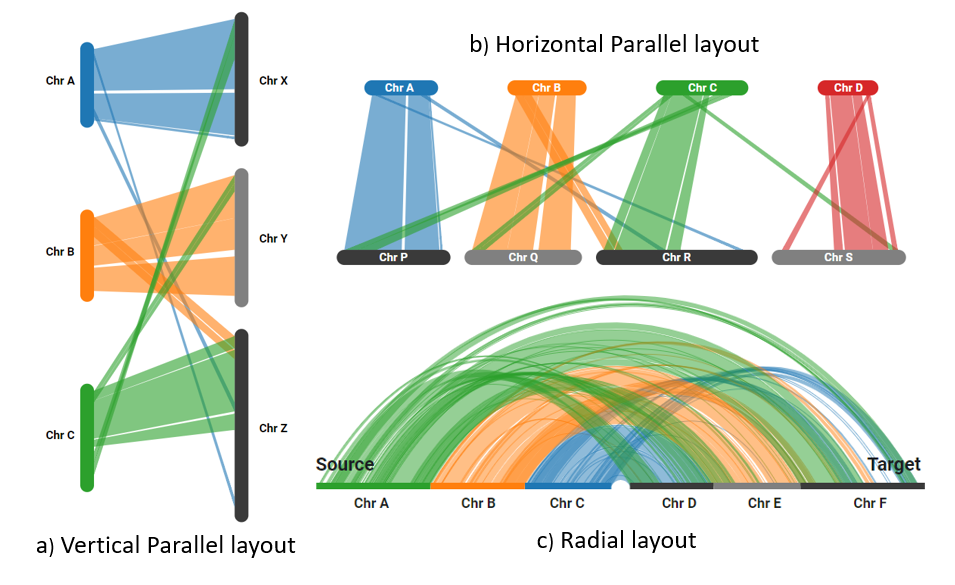
\includegraphics[width=.75\linewidth]{images/ch_4_layout.PNG}
  \captionof{figure}{Different layout strategies at the genome level with conservation being encoded as connections.}
  \label{fig:ch_4_layout}
\end{figure}


In arriving at the optimal layout strategy we looked at several different alternatives ways of arranging the chromosomes.In the popular syteny browser MizBee\cite{Meyer2009} the authors provide a taxonomy of the different synteny layouts and broadly classify them into two categories: contiguous and discrete.In the former the chromosomes are presented adjacent to each other either in a linear or a circular layout and in the later chromosomes are treated as distinct elements and presented either in segregated groups or interleaved with each other.In our design we go for the contiguous scheme but we omit the circular layout as it has already been explored in AccuSyn\cite{accusyn}  and instead look at possible linear layout strategies where conservation is encoded through connections as shown in figure \ref{fig:ch_4_layout}.In the vertical(a) and horizontal layouts(b) the underlying strategy is similar except for the orientation of the two parallel layers.However the number of chromosomes in a genome can be numerous as in the case of humans who have 23 and thus cause the vertical layout to be quite long which makes it sub-optimal for most common screen aspect ratios.Thus of the two, the horizontal parallel layout is the preferred mode of encoding synteny.A common advantage of these two layouts is that they can stacked in multiple layers such that chromosomes at every level are linked to both chromosomes above them and also the chromosomes below them as shown in figure \ref{fig:ch_4_layout_multi}.This stacked layout strategy is used to represent syteny in the form of a tree view chart and can be particularly useful in scenarios where conserved regions need to be traced across several evolutionary levels.

The bi-directional linking strategy is however unavailable in the parallel layout scheme in pairwise comparisons scenarios but can utilized by moving the two layers adjacent to each other as shown by the layout(c) in Figure \ref{fig:ch_4_layout}.In this layout the chromosomes are in the same level thus making it possible for conserved regions to be linked in two directions either from the top or from down below.This gives us an opportunity to add an additional layer of encoding.For example if we had to represent the orientation of the conserved regions we could link all forward matches through connections from top and all reverse matches through connections from the bottom.The disadvantage of this layout is the high number of crossing between the connections.This can be made worse in scenarios where there is a high degree of collinearity between the two genomes due to the ordering of the chromosomes as every connection between the first chromosome in the source and the first chromosome in the target is crossed by all other connections emerging from the rest of the chromosomes in the source.An alternative approach to solve this problem includes reversing the layout of one of the layers or arranging the chromosomes in a radially outwards fashion in  both the layers.This layout can also be extended to express synteny in multiple levels by simply increasing the number of radial layers such that each layer is connected to both the layer on its right and the layer on its left as shown in the layout(b) in Figure \ref{fig:ch_4_layout_multi}.

\begin{figure}
  \centering
  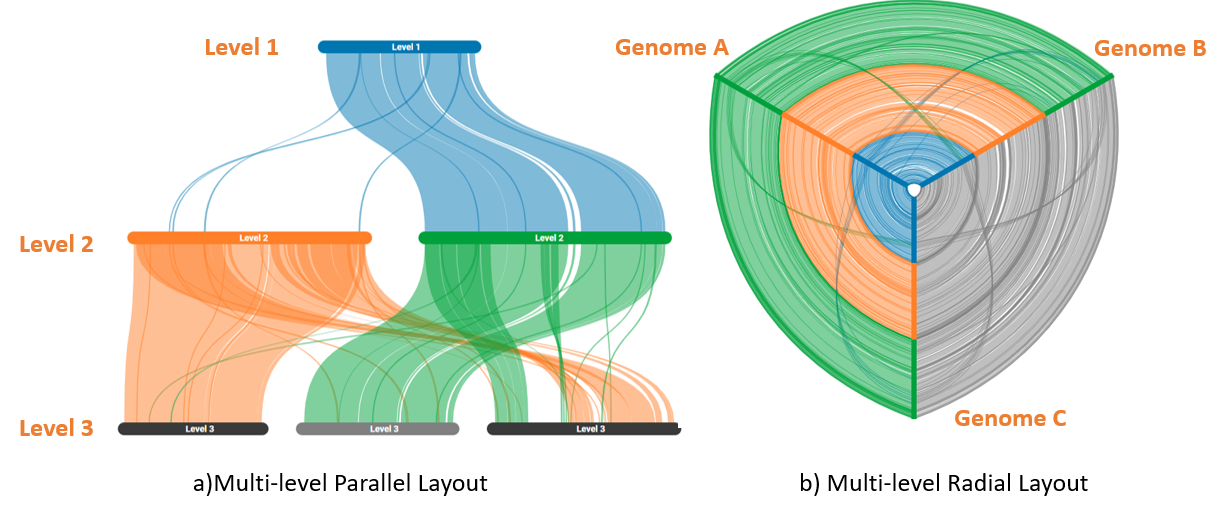
\includegraphics[width=.95\linewidth]{images/ch_4_layout_multi.PNG}
  \captionof{figure}{Multi-level layout strategies.}
  \label{fig:ch_4_layout_multi}
\end{figure}

\section{User Interaction Design}

Having discussed the different ways in which syntenic data can be encoded we can summarise that the usefulness of a particular representation depends on the syntenic relationship under investigation.This has created a need for an adaptive system that can be used under a wide range of scenarios spanning investigation of micro syteny all the way up to high level genome duplication events.Syntenic data also goes beyond the basic location,size and orientation of the conserved regions and includes additional information such as the the match score and the E (expect)value which indicate the level of similarity and the probability of a match occurring by chance respectively.This inherent complexity in the dataset means that exploring it becomes difficult as the volume of the data increases.Thus in designing our syteny exploration interface we build on the framework of the Visual Information Seeking Mantra \cite{Shneiderman96theeyes}.Our design framework breaks down synteny analysis broadly into the following tasks: overview, filter, zoom, details-on-demand , history and extract.

We presents information in a top-down tiered approach in three distinct levels starting with the whole genome followed by stepping down into an individual chromosome and finally ending on the gene block level.Users are giving the ability to start their investigation of the data at any particular level and pick either a dot plot or a parallel plot or combination of both.They can then switch between the levels or drill down into the data by interacting with the visualizations in real time as shown in figure \ref{fig:ch_4_layout_multi}.Additional details about the syntenic blocks are available on demand through hover based mouse interactions either with the ribbons or the dots based on the type of representation.

Our design also incorporates an exploratory dashboard where instead of relying on a single visualization, information about conservation at every level is presented through coordinated multiple views.This is built on the underlying premise that users have a better understanding of their data if they interact with the presented information and view it through different representations\cite{Roberts}.In our design of multiple distinct views that support the investigation of a single entity we followed the design guidelines set by earlier research into multiple views in information visualization systems\cite{WangBaldonado}.We present the following three distinct views each highlighting a unique facet of the dataset : Parallel plot, Dot matrix plot and a simple scatter plot that acts as a filter toggle.The parallel plot offers position and location information about the conserved regions at a glance while the dot matrix plot can easily highlight reversals and deletions within the conserved regions.Both the views are linked to each other in such a way that any interaction in one view such as zooming in and looking at one chromosome is also reflected in the other view ensuring that the user doesn't lose context. The final scatter plot is used to present the measure of similarity of the conserved regions and has a slider built into it that can be used to filter conserved regions based on their match score or E value.The filter works synchronously with the other two views and as the user moves the slider, the conserved regions are filtered in real time in the other two views.Finally in keeping with the visual information seeking mantra framework user interactions are recorded with users having the ability to store all their interactions in arriving at a particular analysis point as a visual stamp that can be revisited again or reset back to in-case of further analysis.

\section{Iterative Development}
By following the guidelines of a standard design study methodology\cite{5290695} our system design occurred iteratively through 4 main development cycles.At every stage we presented our system to a panel composed of genome researchers and information visualization experts to gather feedback and look at possible avenues of improvement.

1st cycle - after the intial requirement gather phase we sketched a prototype of a basic linear parallel plot to represent synteny and developed it.Our inital application was developed as a web application that rendered images on canvas. we found that this had scalability issues and included complexity in linking user interactions with the images. Our choice of colours was bad and made it hard to distinguish the different visual elements.Its easier to group elements on screen into blocks at larger levels.add curves seperate chromosomes.

2nd cycle - Moved to svg and added interactions on the visualizations and additional user interactions in terms of filtering and ability to select chromosomes.hacing to constantly swithc between plots when looking for additional information.critc choice - slider wasnt intuitive and lacked context during filtering.

3rd cycle - base dashboard with all the information. but no way to select multiple comparisions. adding tracks. visual timestamping. Walking into a maze and arriving at the right spot but not knwoing how to comeback. no export or history of user interactions.
